\documentclass{standalone}
\usepackage{tikz}
\usetikzlibrary{patterns, positioning}
\usepackage[sfdefault]{ClearSans} %% option 'sfdefault' activates Clear Sans as the default text font
\usepackage[T1]{fontenc}

\begin{document}
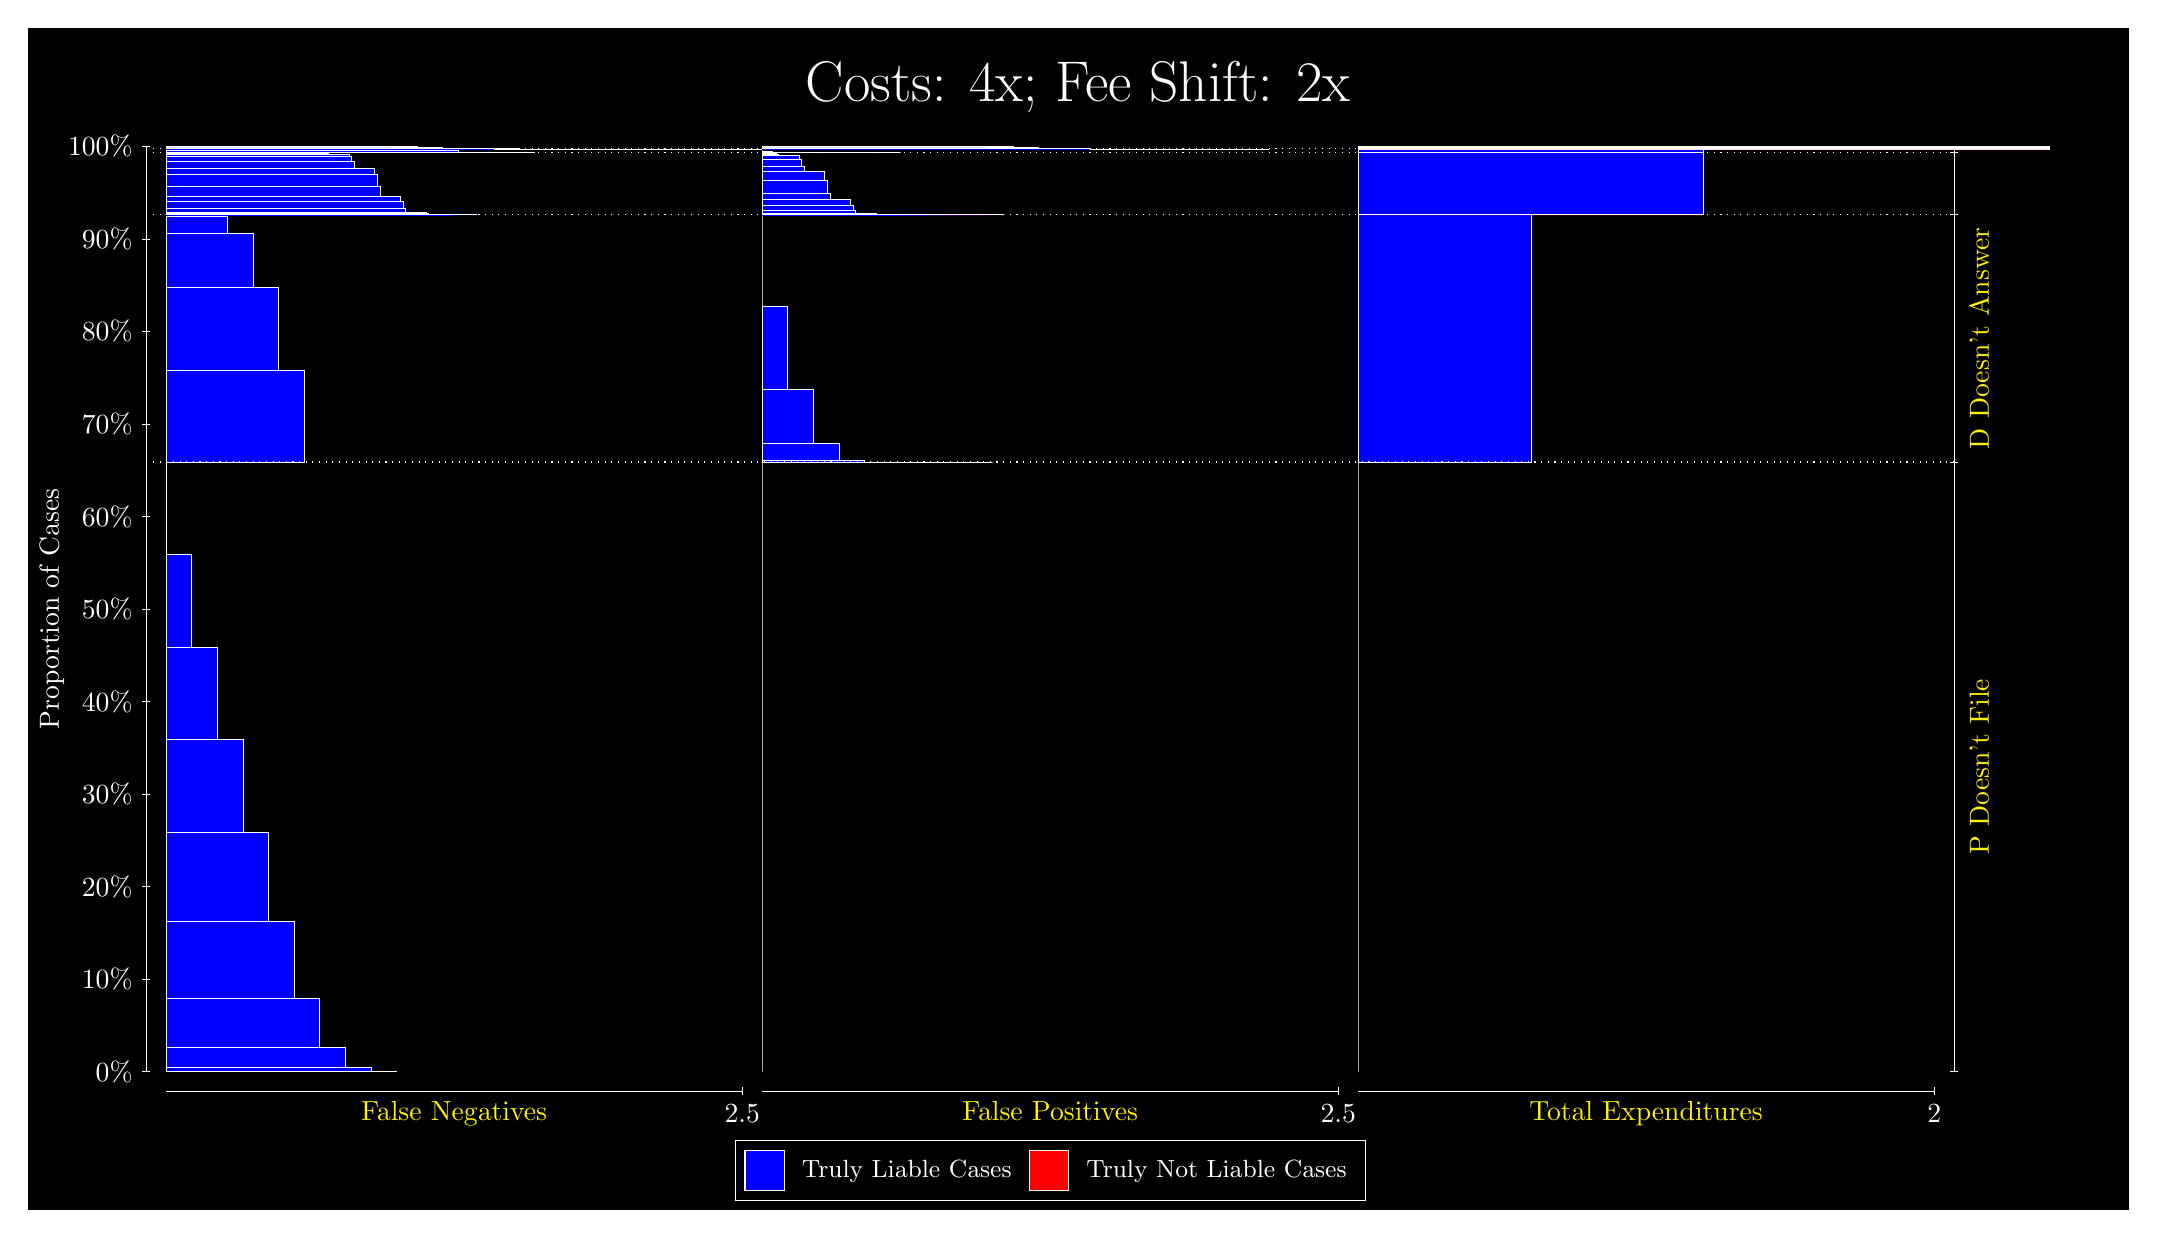
\begin{tikzpicture}
\draw[fill=black] (0,0) rectangle (26.667,15);
\draw[text=white] (0,13.5) rectangle (26.667,15) node[midway] {\huge Costs: 4x; Fee Shift: 2x};
\draw[white, very thin] (1.5,1.75) -- (1.5,13.5);
\node[rotate=90, text=white, anchor=center] at (0.3, 7.625) {Proportion of Cases};
\draw[white, very thin] (1.45,1.75) -- (1.55,1.75);
\node[text=white, anchor=east] at (1.45, 1.75) {0\%};
\draw[white, very thin] (1.45,2.925) -- (1.55,2.925);
\node[text=white, anchor=east] at (1.45, 2.925) {10\%};
\draw[white, very thin] (1.45,4.1) -- (1.55,4.1);
\node[text=white, anchor=east] at (1.45, 4.1) {20\%};
\draw[white, very thin] (1.45,5.275) -- (1.55,5.275);
\node[text=white, anchor=east] at (1.45, 5.275) {30\%};
\draw[white, very thin] (1.45,6.45) -- (1.55,6.45);
\node[text=white, anchor=east] at (1.45, 6.45) {40\%};
\draw[white, very thin] (1.45,7.625) -- (1.55,7.625);
\node[text=white, anchor=east] at (1.45, 7.625) {50\%};
\draw[white, very thin] (1.45,8.8) -- (1.55,8.8);
\node[text=white, anchor=east] at (1.45, 8.8) {60\%};
\draw[white, very thin] (1.45,9.975) -- (1.55,9.975);
\node[text=white, anchor=east] at (1.45, 9.975) {70\%};
\draw[white, very thin] (1.45,11.15) -- (1.55,11.15);
\node[text=white, anchor=east] at (1.45, 11.15) {80\%};
\draw[white, very thin] (1.45,12.325) -- (1.55,12.325);
\node[text=white, anchor=east] at (1.45, 12.325) {90\%};
\draw[white, very thin] (1.45,13.5) -- (1.55,13.5);
\node[text=white, anchor=east] at (1.45, 13.5) {100\%};

\draw[white, very thin] (24.457,1.75) -- (24.457,13.5);
\draw[white, very thin] (24.407,1.75) -- (24.507,1.75);
\node[anchor=west] at (24.407, 1.75) {};
\draw[white, very thin] (24.407,9.4905) -- (24.507,9.4905);
\node[anchor=west] at (24.407, 9.4905) {};
\draw[white, very thin] (24.407,12.631) -- (24.507,12.631);
\node[anchor=west] at (24.407, 12.631) {};
\draw[white, very thin] (24.407,13.422) -- (24.507,13.422);
\node[anchor=west] at (24.407, 13.422) {};
\draw[white, very thin] (24.407,13.467) -- (24.507,13.467);
\node[anchor=west] at (24.407, 13.467) {};
\draw[white, very thin] (24.407,13.5) -- (24.507,13.5);
\node[anchor=west] at (24.407, 13.5) {};

\draw[white, very thin, fill=blue] (1.75,1.75) rectangle (4.6775,1.7563);
\draw[white, very thin, fill=blue] (1.75,1.7563) rectangle (4.3523,1.8085);
\draw[white, very thin, fill=blue] (1.75,1.8085) rectangle (4.027,2.0538);
\draw[white, very thin, fill=blue] (1.75,2.0538) rectangle (3.7017,2.6782);
\draw[white, very thin, fill=blue] (1.75,2.6782) rectangle (3.3764,3.656);
\draw[white, very thin, fill=blue] (1.75,3.656) rectangle (3.0511,4.7939);
\draw[white, very thin, fill=blue] (1.75,4.7939) rectangle (2.7258,5.9657);
\draw[white, very thin, fill=blue] (1.75,5.9657) rectangle (2.4006,7.1406);
\draw[white, very thin, fill=blue] (1.75,7.1406) rectangle (2.0753,8.3156);
\draw[white, very thin, fill=red] (1.75,8.3156) rectangle (1.75,8.3156);
\draw[white, very thin, fill=blue] (1.75,8.3156) rectangle (1.75,9.4905);
\draw[white, very thin, fill=blue] (1.75,9.4905) rectangle (3.5065,10.651);
\draw[white, very thin, fill=blue] (1.75,10.651) rectangle (3.1812,11.708);
\draw[white, very thin, fill=blue] (1.75,11.708) rectangle (2.856,12.395);
\draw[white, very thin, fill=blue] (1.75,12.395) rectangle (2.5307,12.608);
\draw[white, very thin, fill=blue] (1.75,12.608) rectangle (2.2054,12.63);
\draw[white, very thin, fill=blue] (1.75,12.63) rectangle (1.8801,12.631);
\draw[white, very thin, fill=red] (1.75,12.631) rectangle (1.75,12.631);
\draw[white, very thin, fill=blue] (1.75,12.631) rectangle (1.75,12.631);
\draw[white, very thin, fill=blue] (1.75,12.631) rectangle (5.7022,12.631);
\draw[white, very thin, fill=blue] (1.75,12.631) rectangle (5.4094,12.632);
\draw[white, very thin, fill=blue] (1.75,12.632) rectangle (5.3769,12.632);
\draw[white, very thin, fill=blue] (1.75,12.632) rectangle (5.1167,12.64);
\draw[white, very thin, fill=blue] (1.75,12.64) rectangle (5.0842,12.652);
\draw[white, very thin, fill=blue] (1.75,12.652) rectangle (5.0516,12.665);
\draw[white, very thin, fill=blue] (1.75,12.665) rectangle (4.7914,12.715);
\draw[white, very thin, fill=blue] (1.75,12.715) rectangle (4.7589,12.803);
\draw[white, very thin, fill=blue] (1.75,12.803) rectangle (4.7263,12.867);
\draw[white, very thin, fill=blue] (1.75,12.867) rectangle (4.4661,12.99);
\draw[white, very thin, fill=blue] (1.75,12.99) rectangle (4.4336,13.144);
\draw[white, very thin, fill=blue] (1.75,13.144) rectangle (4.4011,13.222);
\draw[white, very thin, fill=blue] (1.75,13.222) rectangle (4.1408,13.307);
\draw[white, very thin, fill=blue] (1.75,13.307) rectangle (4.1083,13.37);
\draw[white, very thin, fill=blue] (1.75,13.37) rectangle (4.0758,13.398);
\draw[white, very thin, fill=blue] (1.75,13.398) rectangle (3.8155,13.412);
\draw[white, very thin, fill=blue] (1.75,13.412) rectangle (3.783,13.418);
\draw[white, very thin, fill=blue] (1.75,13.418) rectangle (3.7505,13.421);
\draw[white, very thin, fill=blue] (1.75,13.421) rectangle (3.4903,13.422);
\draw[white, very thin, fill=blue] (1.75,13.422) rectangle (3.4577,13.422);
\draw[white, very thin, fill=blue] (1.75,13.422) rectangle (3.4252,13.422);
\draw[white, very thin, fill=blue] (1.75,13.422) rectangle (3.165,13.422);
\draw[white, very thin, fill=blue] (1.75,13.422) rectangle (3.1325,13.422);
\draw[white, very thin, fill=blue] (1.75,13.422) rectangle (3.0999,13.422);
\draw[white, very thin, fill=blue] (1.75,13.422) rectangle (2.8397,13.422);
\draw[white, very thin, fill=blue] (1.75,13.422) rectangle (2.8072,13.422);
\draw[white, very thin, fill=blue] (1.75,13.422) rectangle (2.7746,13.422);
\draw[white, very thin, fill=blue] (1.75,13.422) rectangle (2.5144,13.422);
\draw[white, very thin, fill=blue] (1.75,13.422) rectangle (2.4819,13.422);
\draw[white, very thin, fill=blue] (1.75,13.422) rectangle (2.1891,13.422);
\draw[white, very thin, fill=red] (1.75,13.422) rectangle (1.75,13.422);
\draw[white, very thin, fill=blue] (1.75,13.422) rectangle (6.4341,13.422);
\draw[white, very thin, fill=blue] (1.75,13.422) rectangle (6.1088,13.422);
\draw[white, very thin, fill=blue] (1.75,13.422) rectangle (5.7835,13.429);
\draw[white, very thin, fill=blue] (1.75,13.429) rectangle (5.4582,13.45);
\draw[white, very thin, fill=blue] (1.75,13.45) rectangle (5.1329,13.464);
\draw[white, very thin, fill=blue] (1.75,13.464) rectangle (4.8077,13.467);
\draw[white, very thin, fill=blue] (1.75,13.467) rectangle (4.4824,13.467);
\draw[white, very thin, fill=blue] (1.75,13.467) rectangle (4.1571,13.467);
\draw[white, very thin, fill=blue] (1.75,13.467) rectangle (3.8318,13.467);
\draw[white, very thin, fill=blue] (1.75,13.467) rectangle (3.5065,13.467);
\draw[white, very thin, fill=red] (1.75,13.467) rectangle (1.75,13.467);
\draw[white, very thin, fill=blue] (1.75,13.467) rectangle (15.217,13.467);
\draw[white, very thin, fill=blue] (1.75,13.467) rectangle (14.891,13.467);
\draw[white, very thin, fill=blue] (1.75,13.467) rectangle (14.566,13.467);
\draw[white, very thin, fill=blue] (1.75,13.467) rectangle (14.241,13.467);
\draw[white, very thin, fill=blue] (1.75,13.467) rectangle (14.241,13.467);
\draw[white, very thin, fill=blue] (1.75,13.467) rectangle (13.916,13.467);
\draw[white, very thin, fill=blue] (1.75,13.467) rectangle (13.59,13.467);
\draw[white, very thin, fill=blue] (1.75,13.467) rectangle (13.265,13.467);
\draw[white, very thin, fill=blue] (1.75,13.467) rectangle (13.265,13.467);
\draw[white, very thin, fill=blue] (1.75,13.467) rectangle (12.94,13.467);
\draw[white, very thin, fill=blue] (1.75,13.467) rectangle (12.614,13.467);
\draw[white, very thin, fill=blue] (1.75,13.467) rectangle (12.289,13.467);
\draw[white, very thin, fill=blue] (1.75,13.467) rectangle (11.964,13.467);
\draw[white, very thin, fill=blue] (1.75,13.467) rectangle (11.639,13.467);
\draw[white, very thin, fill=blue] (1.75,13.467) rectangle (7.2148,13.467);
\draw[white, very thin, fill=blue] (1.75,13.467) rectangle (6.8895,13.467);
\draw[white, very thin, fill=blue] (1.75,13.467) rectangle (6.5642,13.467);
\draw[white, very thin, fill=blue] (1.75,13.467) rectangle (6.2389,13.469);
\draw[white, very thin, fill=blue] (1.75,13.469) rectangle (5.9136,13.469);
\draw[white, very thin, fill=blue] (1.75,13.469) rectangle (5.9136,13.472);
\draw[white, very thin, fill=blue] (1.75,13.472) rectangle (5.5883,13.476);
\draw[white, very thin, fill=blue] (1.75,13.476) rectangle (5.5883,13.48);
\draw[white, very thin, fill=blue] (1.75,13.48) rectangle (5.2631,13.489);
\draw[white, very thin, fill=blue] (1.75,13.489) rectangle (4.9378,13.492);
\draw[white, very thin, fill=blue] (1.75,13.492) rectangle (4.9378,13.496);
\draw[white, very thin, fill=blue] (1.75,13.496) rectangle (4.6125,13.496);
\draw[white, very thin, fill=blue] (1.75,13.496) rectangle (4.6125,13.499);
\draw[white, very thin, fill=blue] (1.75,13.499) rectangle (4.6125,13.499);
\draw[white, very thin, fill=blue] (1.75,13.499) rectangle (4.2872,13.499);
\draw[white, very thin, fill=blue] (1.75,13.499) rectangle (4.2872,13.5);
\draw[white, very thin, fill=blue] (1.75,13.5) rectangle (3.9619,13.5);
\draw[white, very thin, fill=blue] (1.75,13.5) rectangle (3.6366,13.5);
\draw[white, very thin, fill=blue] (1.75,13.5) rectangle (3.3114,13.5);
\draw[white, very thin, fill=blue] (1.75,13.5) rectangle (3.3114,13.5);
\draw[white, very thin, fill=blue] (1.75,13.5) rectangle (2.9861,13.5);
\draw[white, very thin, fill=blue] (1.75,13.5) rectangle (2.9861,13.5);
\draw[white, very thin, fill=blue] (1.75,13.5) rectangle (2.6608,13.5);
\draw[white, very thin, fill=blue] (1.75,13.5) rectangle (2.6608,13.5);
\draw[white, very thin, fill=blue] (1.75,13.5) rectangle (2.3355,13.5);
\draw[white, very thin, fill=red] (1.75,13.5) rectangle (1.75,13.5);
\draw[white, very thin, fill=red] (9.3189,1.75) rectangle (9.3189,1.75);
\draw[white, very thin, fill=blue] (9.3189,1.75) rectangle (9.3189,9.4905);
\draw[white, very thin, fill=red] (9.3189,9.4905) rectangle (12.246,9.4905);
\draw[white, very thin, fill=blue] (9.3189,9.4905) rectangle (12.246,9.4905);
\draw[white, very thin, fill=blue] (9.3189,9.4905) rectangle (11.921,9.4905);
\draw[white, very thin, fill=blue] (9.3189,9.4905) rectangle (11.596,9.4905);
\draw[white, very thin, fill=blue] (9.3189,9.4905) rectangle (11.271,9.4905);
\draw[white, very thin, fill=blue] (9.3189,9.4905) rectangle (10.945,9.4912);
\draw[white, very thin, fill=blue] (9.3189,9.4912) rectangle (10.62,9.5141);
\draw[white, very thin, fill=blue] (9.3189,9.5141) rectangle (10.295,9.7266);
\draw[white, very thin, fill=blue] (9.3189,9.7266) rectangle (9.9694,10.414);
\draw[white, very thin, fill=blue] (9.3189,10.414) rectangle (9.6442,11.471);
\draw[white, very thin, fill=blue] (9.3189,11.471) rectangle (9.3189,12.631);
\draw[white, very thin, fill=red] (9.3189,12.631) rectangle (12.393,12.631);
\draw[white, very thin, fill=blue] (9.3189,12.631) rectangle (12.393,12.631);
\draw[white, very thin, fill=red] (9.3189,12.631) rectangle (12.1,12.631);
\draw[white, very thin, fill=blue] (9.3189,12.631) rectangle (12.1,12.631);
\draw[white, very thin, fill=blue] (9.3189,12.631) rectangle (12.068,12.631);
\draw[white, very thin, fill=red] (9.3189,12.631) rectangle (11.807,12.631);
\draw[white, very thin, fill=blue] (9.3189,12.631) rectangle (11.807,12.631);
\draw[white, very thin, fill=blue] (9.3189,12.631) rectangle (11.775,12.631);
\draw[white, very thin, fill=blue] (9.3189,12.631) rectangle (11.742,12.631);
\draw[white, very thin, fill=blue] (9.3189,12.631) rectangle (11.482,12.631);
\draw[white, very thin, fill=blue] (9.3189,12.631) rectangle (11.449,12.631);
\draw[white, very thin, fill=blue] (9.3189,12.631) rectangle (11.417,12.631);
\draw[white, very thin, fill=blue] (9.3189,12.631) rectangle (11.157,12.631);
\draw[white, very thin, fill=blue] (9.3189,12.631) rectangle (11.124,12.631);
\draw[white, very thin, fill=blue] (9.3189,12.631) rectangle (11.092,12.632);
\draw[white, very thin, fill=blue] (9.3189,12.632) rectangle (10.831,12.635);
\draw[white, very thin, fill=blue] (9.3189,12.635) rectangle (10.799,12.641);
\draw[white, very thin, fill=blue] (9.3189,12.641) rectangle (10.766,12.655);
\draw[white, very thin, fill=blue] (9.3189,12.655) rectangle (10.506,12.683);
\draw[white, very thin, fill=blue] (9.3189,12.683) rectangle (10.474,12.746);
\draw[white, very thin, fill=blue] (9.3189,12.746) rectangle (10.441,12.831);
\draw[white, very thin, fill=blue] (9.3189,12.831) rectangle (10.181,12.909);
\draw[white, very thin, fill=blue] (9.3189,12.909) rectangle (10.148,13.063);
\draw[white, very thin, fill=blue] (9.3189,13.063) rectangle (10.116,13.186);
\draw[white, very thin, fill=blue] (9.3189,13.186) rectangle (9.8556,13.25);
\draw[white, very thin, fill=blue] (9.3189,13.25) rectangle (9.8231,13.338);
\draw[white, very thin, fill=blue] (9.3189,13.338) rectangle (9.7905,13.388);
\draw[white, very thin, fill=blue] (9.3189,13.388) rectangle (9.5303,13.401);
\draw[white, very thin, fill=blue] (9.3189,13.401) rectangle (9.4978,13.413);
\draw[white, very thin, fill=blue] (9.3189,13.413) rectangle (9.4652,13.421);
\draw[white, very thin, fill=blue] (9.3189,13.421) rectangle (9.3189,13.422);
\draw[white, very thin, fill=red] (9.3189,13.422) rectangle (11.075,13.422);
\draw[white, very thin, fill=blue] (9.3189,13.422) rectangle (11.075,13.422);
\draw[white, very thin, fill=blue] (9.3189,13.422) rectangle (10.75,13.422);
\draw[white, very thin, fill=blue] (9.3189,13.422) rectangle (10.425,13.422);
\draw[white, very thin, fill=blue] (9.3189,13.422) rectangle (10.1,13.422);
\draw[white, very thin, fill=blue] (9.3189,13.422) rectangle (9.7743,13.424);
\draw[white, very thin, fill=blue] (9.3189,13.424) rectangle (9.449,13.439);
\draw[white, very thin, fill=blue] (9.3189,13.439) rectangle (9.3189,13.467);
\draw[white, very thin, fill=red] (9.3189,13.467) rectangle (15.759,13.467);
\draw[white, very thin, fill=blue] (9.3189,13.467) rectangle (15.759,13.467);
\draw[white, very thin, fill=blue] (9.3189,13.467) rectangle (15.434,13.467);
\draw[white, very thin, fill=red] (9.3189,13.467) rectangle (15.434,13.467);
\draw[white, very thin, fill=blue] (9.3189,13.467) rectangle (15.434,13.467);
\draw[white, very thin, fill=red] (9.3189,13.467) rectangle (15.109,13.467);
\draw[white, very thin, fill=blue] (9.3189,13.467) rectangle (15.109,13.467);
\draw[white, very thin, fill=blue] (9.3189,13.467) rectangle (15.109,13.467);
\draw[white, very thin, fill=blue] (9.3189,13.467) rectangle (14.784,13.467);
\draw[white, very thin, fill=red] (9.3189,13.467) rectangle (14.784,13.467);
\draw[white, very thin, fill=blue] (9.3189,13.467) rectangle (14.784,13.467);
\draw[white, very thin, fill=blue] (9.3189,13.467) rectangle (14.784,13.467);
\draw[white, very thin, fill=blue] (9.3189,13.467) rectangle (14.458,13.467);
\draw[white, very thin, fill=red] (9.3189,13.467) rectangle (14.458,13.467);
\draw[white, very thin, fill=blue] (9.3189,13.467) rectangle (14.458,13.467);
\draw[white, very thin, fill=blue] (9.3189,13.467) rectangle (14.458,13.467);
\draw[white, very thin, fill=blue] (9.3189,13.467) rectangle (14.133,13.467);
\draw[white, very thin, fill=red] (9.3189,13.467) rectangle (14.133,13.467);
\draw[white, very thin, fill=blue] (9.3189,13.467) rectangle (14.133,13.467);
\draw[white, very thin, fill=blue] (9.3189,13.467) rectangle (14.133,13.467);
\draw[white, very thin, fill=blue] (9.3189,13.467) rectangle (13.808,13.467);
\draw[white, very thin, fill=blue] (9.3189,13.467) rectangle (13.808,13.467);
\draw[white, very thin, fill=red] (9.3189,13.467) rectangle (13.808,13.467);
\draw[white, very thin, fill=blue] (9.3189,13.467) rectangle (13.808,13.467);
\draw[white, very thin, fill=blue] (9.3189,13.467) rectangle (13.808,13.468);
\draw[white, very thin, fill=blue] (9.3189,13.468) rectangle (13.482,13.469);
\draw[white, very thin, fill=blue] (9.3189,13.469) rectangle (13.482,13.469);
\draw[white, very thin, fill=blue] (9.3189,13.469) rectangle (13.482,13.471);
\draw[white, very thin, fill=blue] (9.3189,13.471) rectangle (13.157,13.475);
\draw[white, very thin, fill=blue] (9.3189,13.475) rectangle (13.157,13.475);
\draw[white, very thin, fill=blue] (9.3189,13.475) rectangle (13.157,13.478);
\draw[white, very thin, fill=blue] (9.3189,13.478) rectangle (12.832,13.485);
\draw[white, very thin, fill=blue] (9.3189,13.485) rectangle (12.832,13.486);
\draw[white, very thin, fill=blue] (9.3189,13.486) rectangle (12.832,13.487);
\draw[white, very thin, fill=blue] (9.3189,13.487) rectangle (12.507,13.494);
\draw[white, very thin, fill=blue] (9.3189,13.494) rectangle (12.507,13.494);
\draw[white, very thin, fill=blue] (9.3189,13.494) rectangle (12.507,13.495);
\draw[white, very thin, fill=blue] (9.3189,13.495) rectangle (12.181,13.495);
\draw[white, very thin, fill=blue] (9.3189,13.495) rectangle (12.181,13.498);
\draw[white, very thin, fill=blue] (9.3189,13.498) rectangle (12.181,13.498);
\draw[white, very thin, fill=blue] (9.3189,13.498) rectangle (11.856,13.498);
\draw[white, very thin, fill=blue] (9.3189,13.498) rectangle (11.856,13.499);
\draw[white, very thin, fill=blue] (9.3189,13.499) rectangle (11.531,13.5);
\draw[white, very thin, fill=blue] (9.3189,13.5) rectangle (11.531,13.5);
\draw[white, very thin, fill=blue] (9.3189,13.5) rectangle (11.206,13.5);
\draw[white, very thin, fill=blue] (9.3189,13.5) rectangle (10.88,13.5);
\draw[white, very thin, fill=red] (9.3189,13.5) rectangle (9.3189,13.5);
\draw[white, very thin, fill=blue] (9.3189,13.5) rectangle (9.3189,13.5);
\draw[white, very thin, fill=red] (16.888,1.75) rectangle (16.888,1.75);
\draw[white, very thin, fill=blue] (16.888,1.75) rectangle (16.888,9.4905);
\draw[white, very thin, fill=red] (16.888,9.4905) rectangle (19.083,9.4905);
\draw[white, very thin, fill=blue] (16.888,9.4905) rectangle (19.083,12.631);
\draw[white, very thin, fill=red] (16.888,12.631) rectangle (21.279,12.631);
\draw[white, very thin, fill=blue] (16.888,12.631) rectangle (21.279,13.422);
\draw[white, very thin, fill=red] (16.888,13.422) rectangle (21.279,13.422);
\draw[white, very thin, fill=blue] (16.888,13.422) rectangle (21.279,13.467);
\draw[white, very thin, fill=red] (16.888,13.467) rectangle (25.67,13.467);
\draw[white, very thin, fill=blue] (16.888,13.467) rectangle (25.67,13.47);
\draw[white, very thin, fill=red] (16.888,13.47) rectangle (25.67,13.47);
\draw[white, very thin, fill=blue] (16.888,13.47) rectangle (25.67,13.494);
\draw[white, very thin, fill=red] (16.888,13.494) rectangle (25.67,13.494);
\draw[white, very thin, fill=blue] (16.888,13.494) rectangle (25.67,13.5);
\draw[white, dotted] (1.5,9.4905) -- (24.457,9.4905);
\draw[white, dotted] (1.5,12.631) -- (24.457,12.631);
\draw[white, dotted] (1.5,13.422) -- (24.457,13.422);
\draw[white, dotted] (1.5,13.467) -- (24.457,13.467);
\draw[white, very thin] (1.75,1.5) -- (9.0689,1.5);
\node[text=yellow, anchor=north] at (5.4094, 1.5) {False Negatives};
\draw[white, very thin] (9.0689,1.45) -- (9.0689,1.55);
\node[text=white, anchor=north] at (9.0689, 1.45) {2.5};

\draw[white, very thin] (9.3189,1.5) -- (16.638,1.5);
\node[text=yellow, anchor=north] at (12.978, 1.5) {False Positives};
\draw[white, very thin] (16.638,1.45) -- (16.638,1.55);
\node[text=white, anchor=north] at (16.638, 1.45) {2.5};

\draw[white, very thin] (16.888,1.5) -- (24.207,1.5);
\node[text=yellow, anchor=north] at (20.547, 1.5) {Total Expenditures};
\draw[white, very thin] (24.207,1.45) -- (24.207,1.55);
\node[text=white, anchor=north] at (24.207, 1.45) {2};

\node[text=yellow, centered, rotate=90] at (24.777, 5.6203) {P Doesn't File};
\node[text=yellow, centered, rotate=90] at (24.777, 11.061) {D Doesn't Answer};




\draw (12.978300999999998,1.5) node[draw=none] (baseCoordinate) {};
\begin{scope}[align=center]
        \matrix[scale=0.5, draw=white, below=0.5cm of baseCoordinate, nodes={draw}, column sep=0.1cm]{
            \node[rectangle, draw, minimum width=0.5cm, minimum height=0.5cm, fill=blue] {}; &
            \node[draw=none, font=\small, text=white] (B) {Truly Liable Cases}; &
            \node[rectangle, draw, minimum width=0.5cm, minimum height=0.5cm, fill=red] {}; &
            \node[draw=none, font=\small, text=white] (B) {Truly Not Liable Cases}; \\
            };
\end{scope}

\end{tikzpicture}
\end{document}